Given is the continuous signal $s(t)$.

\pgfplotsset{
	axis412/.style={
			clip=false,
			axis lines=middle,
			xmin=-6.5, xmax=6.5,
			xlabel={$t$},
			xtick distance={2},
			ymin=0, ymax=1.3,
			y=2.5cm,
			ylabel={$s(t)$},
			yticklabels={$\hat{s}$},
			ytick={1},
			hide obscured x ticks=false,
			x label style={at={(current axis.right of origin)},	anchor=east, right=1mm},
			y label style={at={(current axis.above origin)}, anchor=south },
			hide obscured x ticks=false
		},
}

\begin{figure}[H]
	\centering
	\begin{tikzpicture}
		\pgfplotsset{
			every axis plot/.append style={line width=1pt, mark=none, samples=10}
		}
		\begin{axis}[axis412,width=12cm, xtick distance={1}]
			\addplot[color=blue] coordinates {(-6,0) (0,0) (0,1) (3,0) (6,0)};
			\addplot[color=gray!60, line width=0.75pt, dashed] coordinates {(0,1) (3,1)  (3,0)};

			\draw node[above] at (1.5, 1) {$3$};
			\draw node[right] at (3, 0.5) {$1$};
		\end{axis}
	\end{tikzpicture}
	\caption{\label{412-1}$s(t)$}
\end{figure}

If $\hat{s} = 1$, the following applies to $s(t)$
\begin{flalign*}
	\quad s(t) = \begin{cases}
		             0, \quad t < 0                     \\
		             \hat{s}=1, \quad t = 0             \\
		             -\frac{1}{3}t + 1, \quad 0 < t < 3 \\
		             0, \quad t > 3
	             \end{cases}
\end{flalign*}

\subsubsection{Solutions}
\begin{tabularx}{\linewidth}{@{}l@{}X@{}@{}l@{}X@{}}
	a)                                &
	\begin{equation*}
		s(-t) = \begin{cases}
			0, \quad t > 0                     \\
			\hat{s}=1, \quad t = 0             \\
			\frac{1}{3}t + 1, \quad -3 < t < 0 \\
			0, \quad t < -3
		\end{cases}
	\end{equation*} &
	b)                                &
	\begin{equation*}
		s(t+2) = \begin{cases}
			0, \quad t < -2                               \\
			\hat{s}=1, \quad t = -2                       \\
			-\frac{1}{3}t + \frac{1}{3}, \quad -2 < t < 1 \\
			0, \quad t \geq 1
		\end{cases}
	\end{equation*}   \\
	                                  &
	\begin{tikzpicture}
		\begin{axis}[axis412]
			\addplot[color=blue] coordinates {(-6,0) (-3,0) (0,1) (0,0) (6,0)};
		\end{axis}
	\end{tikzpicture}         &

	                                  &
	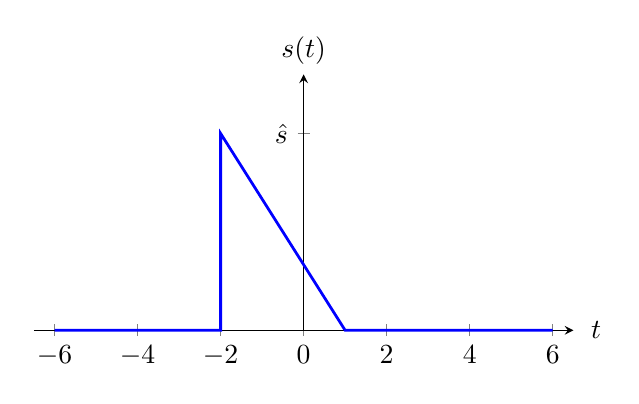
\begin{tikzpicture}
		\begin{axis}[axis412]
			\addplot[color=blue] coordinates {(-6,0) (-2,0) (-2,1) (1,0) (6,0)};
		\end{axis}
	\end{tikzpicture}
\end{tabularx}

\begin{tabularx}{\linewidth}{@{}l@{}X@{}@{}l@{}X@{}}
	c)                                  &
	\begin{equation*}
		s(2t+2) = \begin{cases}
			0, \quad t < -1                                         \\
			\hat{s}=1, \quad t = -1                                 \\
			-\frac{2}{3}t + \frac{1}{3}, \quad -1 < t < \frac{1}{2} \\
			0, \quad t \geq \frac{1}{2}
		\end{cases}
	\end{equation*} &
	d)                                  &
	\begin{equation*}
		s(1-3t) = \begin{cases}
			0, \quad t \leq -\frac{2}{3}                           \\
			t+\frac{2}{3}, \quad -\frac{2}{3} \leq t < \frac{1}{3} \\
			\hat{s}=1, \quad t = \frac{1}{3}                       \\
			0, \quad t \geq \frac{1}{3}
		\end{cases}
	\end{equation*}    \\
	                                    &
	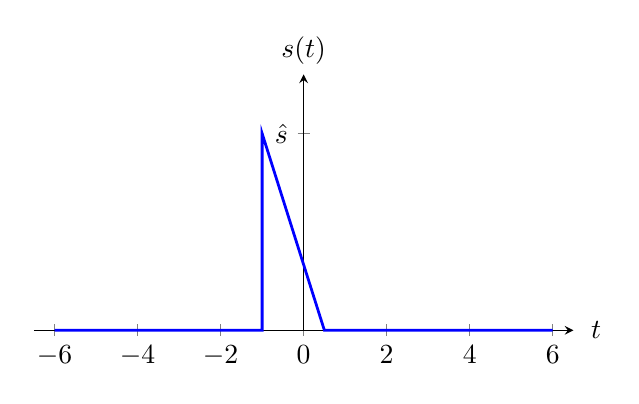
\begin{tikzpicture}
		\begin{axis}[axis412]
			\addplot[color=blue] coordinates {(-6,0) (-1,0) (-1,1) (1/2,0) (6,0)};
		\end{axis}
	\end{tikzpicture}          &
	                                    &
	\begin{tikzpicture}
		\begin{axis}[axis412]
			\addplot[color=blue] coordinates {(-6,0) (-2/3,0) (1/3,1) (1/3,0) (6,0)};
		\end{axis}
	\end{tikzpicture}
\end{tabularx}

\subsubsection{Matlab}
\lstinputlisting[language=Matlab]{./assets/Lab1_412.m}
{
	\setlength{\fboxsep}{0pt}%  
	\colorbox{backcolor}{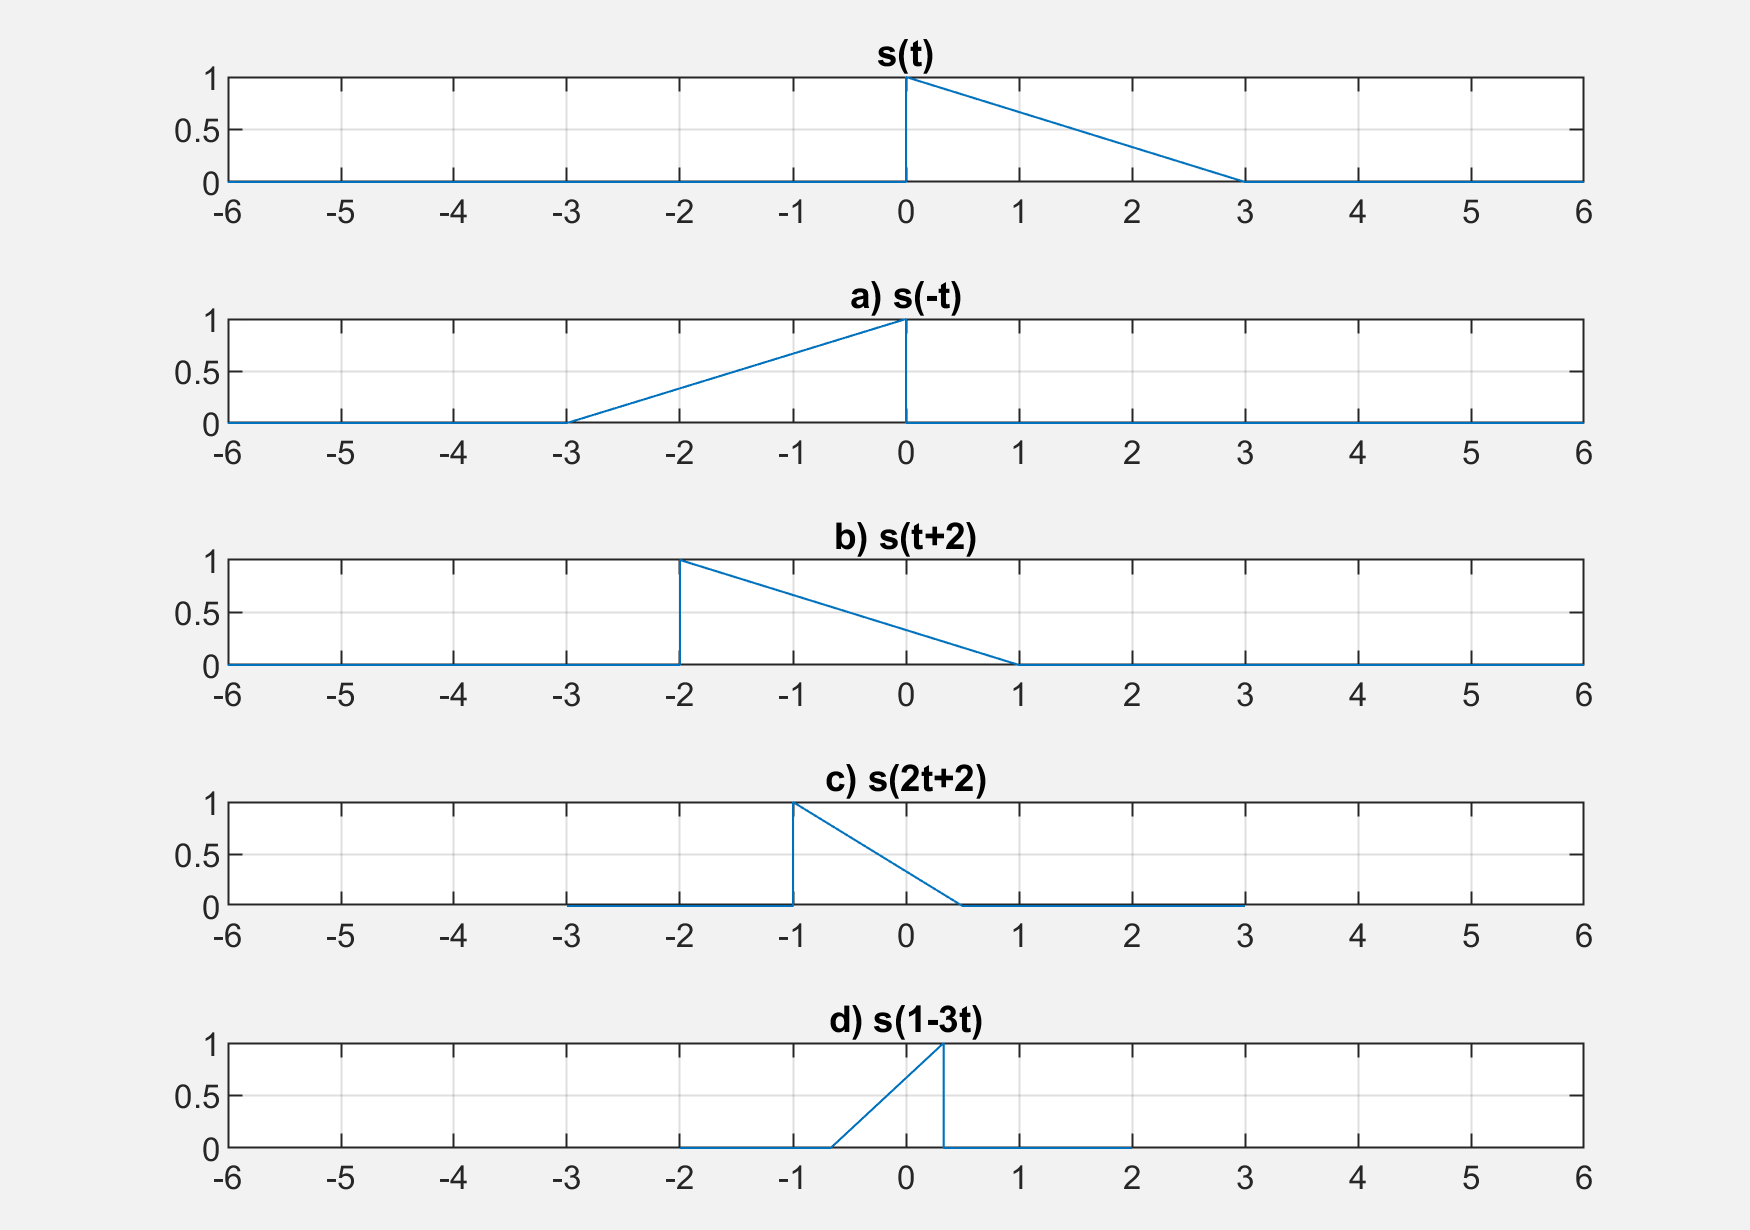
\includegraphics[width=\linewidth, keepaspectratio]{./assets/412.png}}
}